\documentclass[24pt,pdf,hyperref={unicode},aspectratio=169]{beamer}
\usepackage[utf8]{inputenc}
\usepackage{aiml}
\begin{document}


\section{Язык логики высказываний}

\begin{frame}\frametitle{Пропозициональные связки }

$$
\uncover<10->{\overline{0}=}\neg 0=1,\ \uncover<10->{\overline{1}=}\neg 1=0
$$

\uncover<3->
{
$$
\begin{array}{c c c c c c c c c c c}
A & B &  \uncover<4->{A\wedge B} & \uncover<5->{A\vee B}& \uncover<6->{A\rightarrow B}& \uncover<7->{A\oplus B}& \uncover<8->{A\leftrightarrow B}& \uncover<9->{A\uparrow B}& \uncover<11->{A|B} \\
0 & 0 &  \uncover<4->{0}& \uncover<5->{0}& \uncover<6->{1}& \uncover<7->{0}& \uncover<8->{1}& \uncover<9->{1}& \uncover<11->{1} \\
0 & 1 &  \uncover<4->{0}& \uncover<5->{1}& \uncover<6->{1}& \uncover<7->{1}& \uncover<8->{0}& \uncover<9->{0}& \uncover<11->{1} \\
1 & 0 &  \uncover<4->{0}& \uncover<5->{1}& \uncover<6->{0}& \uncover<7->{1}& \uncover<8->{0}& \uncover<9->{0}& \uncover<11->{1} \\
1 & 1 &  \uncover<4->{1}& \uncover<5->{1}& \uncover<6->{1}& \uncover<7->{0}& \uncover<8->{1}& \uncover<9->{0}& \uncover<11->{0} \\
\end{array}
$$
}

$
\begin{array}{r c l}
\uncover<6->{A\rightarrow B & = & \neg A \vee B} \\
\uncover<7->{A\oplus B & = & (\neg A \wedge B)\vee(\neg B \wedge A)} \\
\uncover<8->{A\leftrightarrow B & = & (A \rightarrow B)\wedge(B \rightarrow A)} \\
\uncover<9->{A\uparrow B & = & \overline{A\vee B} }\\
\uncover<11->{A| B & = & \overline{A\wedge B} }\\

\end{array}
$


\end{frame}

\section{Логический вывод}

\begin{frame}\frametitle{Modus ponens}
{\huge
$$
\frac{A,\ A\rightarrow B}{B}
$$
}
\end{frame}

\begin{frame}\frametitle{Аксиомы}
\begin{enumerate}
 \item[A1] $A\rightarrow(B\rightarrow A)$
 \item[A2] $\left[A\rightarrow(B\rightarrow C)\right]\rightarrow\left[(A\rightarrow B)\rightarrow(A\rightarrow C)\right]$
 \item[A3] $(\neg A\rightarrow \neg B)\rightarrow\left[(\neg A\rightarrow B)\rightarrow A\right]$
\end{enumerate}
\end{frame}

\begin{frame}\frametitle{$X\rightarrow X$?}
$$
\begin{array}{l l}
\uncover<+->{A2 & \left[A\rightarrow(B\rightarrow C)\right]\rightarrow\left[(A\rightarrow B)\rightarrow(A\rightarrow C)\right]}\\
\uncover<+->{& A=X,\ B=X\rightarrow X,\ C=X}\\
\uncover<+->{L1 & \left[X\rightarrow((X\rightarrow X)\rightarrow X)\right]\rightarrow\left[(X\rightarrow (X\rightarrow X))\rightarrow(X\rightarrow X)\right]}\\
\uncover<+->{A1 & A\rightarrow(B\rightarrow A)} \\
\uncover<+->{& A=X,\ B=X\rightarrow X}\\
\uncover<+->{L2 & X\rightarrow((X\rightarrow X) \rightarrow X)} \\
\uncover<+->{MP & (X\rightarrow (X\rightarrow X))\rightarrow(X\rightarrow X)} \\
\uncover<+->{A1 & A\rightarrow(B\rightarrow A)} \\
\uncover<+->{& A=X,\ B=X}\\
\uncover<+->{L3 & X\rightarrow (X\rightarrow X)} \\
\uncover<+->{MP & X\rightarrow X}
\end{array}
$$
\end{frame}

\begin{frame}\frametitle{Вывод таблиц истинности}
\begin{itemize}[<+->]
\item $X\rightarrow X \uncover<+->{\ \Rightarrow\ \neg A\rightarrow \neg A} \uncover<+->{\ \Rightarrow\ \neg(A)\rightarrow(\neg A)}$
\item $X\rightarrow \neg\neg X \uncover<+->{}\uncover<+->{\ \Rightarrow\ A\rightarrow \neg\neg A}\uncover<+->{\ \Rightarrow\ A\rightarrow \neg(\neg A)}$
\end{itemize}

\only<5>
{
\begin{center}
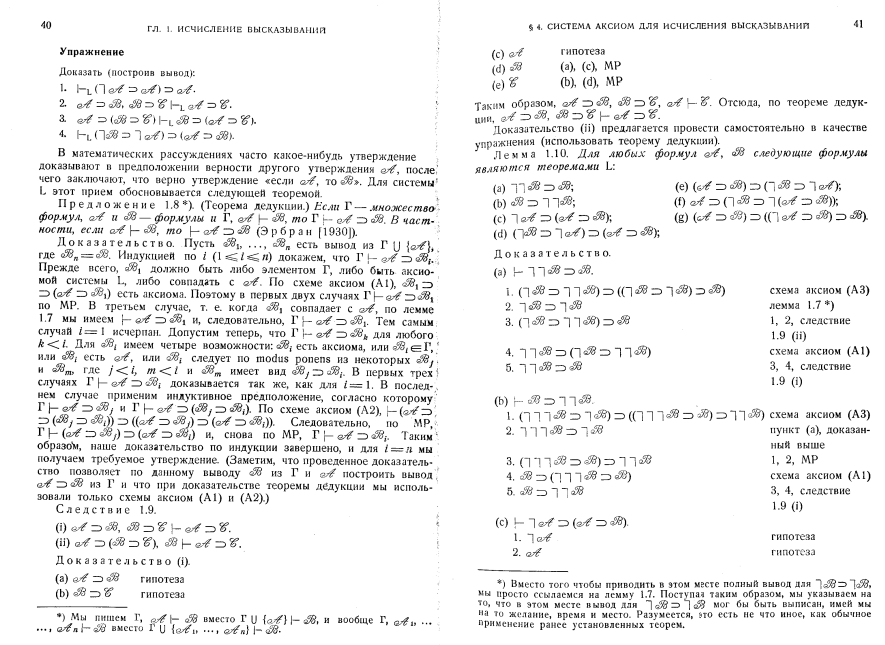
\includegraphics[width=9cm]{Mendelson.png}

(Э. Мендельсон, Введение в математическую логику, с. 40-41)
\end{center}
}

\uncover<+->{
$$
\begin{array}{c|c}
A & \neg A \\
\hline
\uncover<+->{0 & 1} \\
\uncover<+->{1 & 0} \\
\end{array}
$$
}

\begin{itemize}[<+->]
\item $A\rightarrow(B\rightarrow A)$
\item $\neg X\rightarrow (X\rightarrow Y) {\ \Rightarrow\ \neg A\rightarrow(A\rightarrow B)}$
\item $A\rightarrow(\neg B\rightarrow\neg(A\rightarrow B))$
\end{itemize}
\uncover<+->{
$$
\begin{array}{c c| c}
A & B & A\rightarrow B \\
\hline
\uncover<+->{0 & 0 & 1} \\
\uncover<+->{0 & 1 & 1} \\
\uncover<+->{1 & 0 & 0} \\
\uncover<+->{1 & 1 & 1} \\
\end{array}
$$
}
\end{frame}

\begin{frame}\frametitle{Вывод таблиц истинности}
\begin{itemize}[<+->]
\item $A\vee B:=\neg A\rightarrow B$

\uncover<+->{
$$
\begin{array}{c c|c |c}
A & B & \neg A & \neg A\rightarrow B=A\vee B \\
\hline
0 & 0 & 1 & 0 \\
0 & 1 & 1 & 1 \\
1 & 0 & 0 & 1 \\
1 & 1 & 0 & 1 \\
\end{array}
$$
}

\item $A\wedge B:=\neg(A\rightarrow \neg B)$

\uncover<+->{
$$
\begin{array}{c c| c| c| c}
A & B & \neg B & A\rightarrow \neg B & \neg(A\rightarrow\neg B) =A\wedge B \\
\hline
0 & 0 & 1 & 1 & 0 \\
0 & 1 & 0 & 1 & 0\\
1 & 0 & 1 & 1 & 0\\
1 & 1 & 0 & 0 & 1\\
\end{array}
$$
}
\end{itemize}
\end{frame}

\section{Законы логики высказываний}

\begin{frame}\frametitle{Эквивалентность высказываний}
$$
\overline{A}\wedge\overline{B}=\overline{A\vee B}\only<1-7>{?}\only<8>{!}
$$

\uncover<2->{
$$
\begin{array}{c c|c|c|c|c|c}
A & B & \overline{A} & \overline{B} & \overline{A}\wedge\overline{B} & A\vee B & \overline{A\vee B} \\
\hline
0 & 0 & \uncover<3->{1} & \uncover<4->{1} & \uncover<5->{1} & \uncover<6->{0} & \uncover<7->{1} \\
0 & 1 & \uncover<3->{1} & \uncover<4->{0} & \uncover<5->{0} & \uncover<6->{1} & \uncover<7->{0} \\
1 & 0 & \uncover<3->{0} & \uncover<4->{1} & \uncover<5->{0} & \uncover<6->{1} & \uncover<7->{0} \\
1 & 1 & \uncover<3->{0} & \uncover<4->{0} & \uncover<5->{0} & \uncover<6->{1} & \uncover<7->{0} \\
\end{array}
$$
}
\end{frame}

\begin{frame}\frametitle{Эквивалентность высказываний}
\uncover<+->{$$
\overline{A}\wedge\overline{B}=\overline{A\vee B}
$$}
\uncover<+->{$$
(\overline{A}\wedge\overline{B})\leftrightarrow(\overline{A\vee B})
$$}
\uncover<+->{$$
\left[(\overline{A}\wedge\overline{B})\rightarrow(\overline{A\vee B})\right]\wedge
\left[(\overline{A\vee B})\rightarrow(\overline{A}\wedge\overline{B})\right]
$$}
\uncover<+->{$$
\mathcal{L}\vdash
\left[(\overline{A}\wedge\overline{B})\rightarrow(\overline{A\vee B})\right]\wedge
\left[(\overline{A\vee B})\rightarrow(\overline{A}\wedge\overline{B})\right]
$$}
\end{frame}

\begin{frame}\frametitle{Законы логики высказываний}
{\small
$$
\begin{array}{c p{1cm} c}
\multicolumn{3}{c}{$Ассоциативность$} \\
\begin{array}{l}
\ \ \ A\vee (B\vee C)=\\
=(A\vee B)\vee C=\\
=A\vee B\vee C\\
\end{array} &&
\begin{array}{l}
\ \ \ A\wedge (B\wedge C)=\\
=(A\wedge B)\wedge C=\\
=A\wedge B\wedge C\\
\end{array} \\
\multicolumn{3}{c}{$Коммутативность$} \\
A\vee B=B\vee A && A\wedge B=B\wedge A\\
\multicolumn{3}{c}{$Константы и идемпотентность$} \\
A\vee 1=1 && A\wedge 1=A \\
A\vee 0=A && A\wedge 0=0 \\
A\vee A=A && A\wedge A=A \\
\multicolumn{3}{c}{$Дистрибутивность$} \\
A\vee (B\wedge C)= && A\wedge (B\vee C)= \\
=(A\vee C)\wedge (A\vee C) && =(A\wedge B)\vee (A\wedge C) \\
\multicolumn{3}{c}{$Отрицание отрицания$} \\
\multicolumn{3}{c}{\neg\neg A=A} \\
\multicolumn{3}{c}{$Законы де Моргана$} \\
\overline{A\vee B}=\overline{A}\wedge\overline{B}&& \overline{A\wedge B}=\overline{A}\vee\overline{B} \\
\end{array}
$$
}
\end{frame}
\begin{frame}\frametitle{Конъюнктивная нормальная форма}

$$
\begin{array}{l l l}
& (A \vee B \vee C) & \wedge \\
& (\neg A \vee B \vee \neg C) & \wedge \\
& (\neg A)
\end{array}
$$
\end{frame}

\begin{frame}\frametitle{Конъюнктивная нормальная форма}
$$
\begin{array}{l}
\uncover<+->{ \neg A } \\
\uncover<+->{ \neg A \vee B } \\
\uncover<+->{ (A \vee B) \vee C } \uncover<+->{ = A\vee B\vee C }\\
\uncover<+->{ (A\vee B)\wedge C } \\
\uncover<+->{ (A\vee B)\wedge (\neg C\vee D) } \\
\uncover<+->{ (A \wedge B) \vee C } \uncover<+->{ = (A\vee C)\wedge (B\vee C)}\\
\end{array}
$$
\end{frame}

\begin{frame}\frametitle{Приведение к КНФ}
$$
\begin{array}{l}
\uncover<+->{\neg A\rightarrow \overline{B\rightarrow C}}\\
\uncover<+->{ A \vee \overline{\neg B \vee C }} \\
\uncover<+->{ A \vee (B \wedge \neg C) } \\
\uncover<+->{ (A\vee B) \wedge (A \vee \neg C) }
\end{array}
$$
\end{frame}

\section{Метод резолюций}

\begin{frame}\frametitle{Правило резолюций}
{\huge
$$
\frac{A\vee B,\ \neg A \vee C}{B \vee C}
$$
}
\end{frame}

\begin{frame}\frametitle{Правило резолюций}
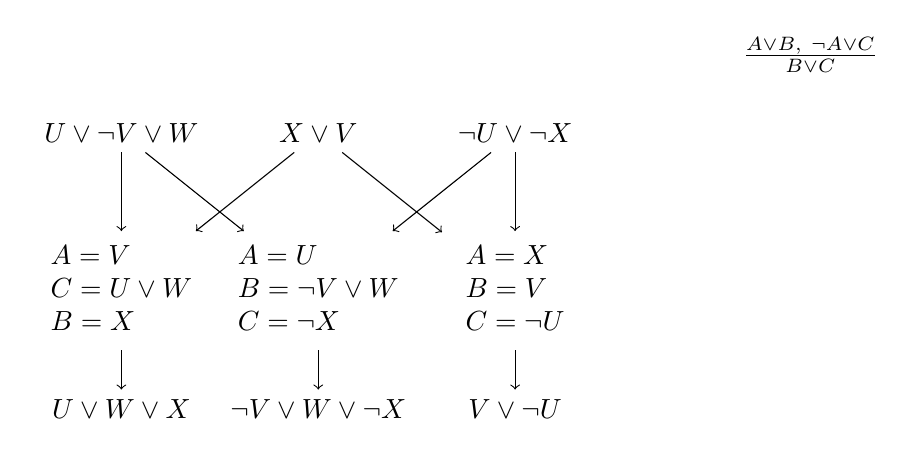
\begin{tikzpicture}[x=2.5cm]
\node at (3.5,4) {$\frac{A\vee B,\ \neg A \vee C}{B \vee C}$};
\node (p1) at (0,3) {$U\vee \neg V \vee W$};
\node (p2) at (1,3) {$X\vee V$};
\node (p3) at (2,3) {$ \neg U\vee \neg X$};

\uncover<2->{
\node (s1) at (0,1) {$\begin{array}{l} A=V\\ C=U\vee W\\ B=X \end{array}$};
\node (r1) at (0,-0.5) {$U\vee W\vee X$};
\path (p1) edge[->] (s1);
\path (p2) edge[->] (s1);
\path (s1) edge[->] (r1);
}

\uncover<3->{
\node (s2) at (1,1) {$\begin{array}{l} A=U\\ B=\neg V \vee W\\ C=\neg X \end{array}$};
\node (r2) at (1,-0.5) {$\neg V\vee W\vee \neg X$};
\path (p1) edge[->] (s2);
\path (p3) edge[->] (s2);
\path (s2) edge[->] (r2);
}

\uncover<4->{
\node (s3) at (2,1) {$\begin{array}{l} A=X\\ B=V \\ C=\neg U \end{array}$};
\node (r3) at (2,-0.5) {$V\vee \neg U$};
\path (p2) edge[->] (s3);
\path (p3) edge[->] (s3);
\path (s3) edge[->] (r3);
}
\end{tikzpicture}
\end{frame}

\begin{frame}\frametitle{Правило резолюций}
\begin{tikzpicture}[x=2.2cm]
\node at (4,4) {$\frac{A\vee B,\ \neg A \vee C}{B \vee C}$};
\node (p2) at (0,3) {$X$};
\node (p1) at (1.5,3) {$\neg X \vee Y \vee Z$};
\node (p3) at (3,3) {$\neg Z$};

\uncover<2->{
\node at (4,3) {$\frac{A\rightarrow B,\ A}{B}$};

\node (t1) at (0.75,2) {$X\rightarrow Y\vee Z$};
\node (s1) at (0.5,0.5) {$\begin{array}{l} A=X\\ B=Y\vee Z\end{array}$};
\node (r1) at (0.5,-1) {$Y\vee Z$};

\path (p1) edge[->] (t1);
\path (t1) edge[->] (s1);
\path (p2) edge[->] (s1);
\path (s1) edge[->] (r1);
}

\uncover<3->{
\node (t2) at (2.25,2) {$\neg Z\rightarrow \neg X\vee Y$};
\node (s2) at (2.5,0.5) {$\begin{array}{l} A=\neg Z\\ B=\neg X \vee Y\end{array}$};
\node (r2) at (2.5,-1) {$\neg X \vee Y$};

\path (p1) edge[->] (t2);
\path (t2) edge[->] (s2);
\path (p3) edge[->] (s2);
\path (s2) edge[->] (r2);
}

\end{tikzpicture}
\end{frame}

\begin{frame}\frametitle{Правило резолюций}
\begin{tikzpicture}[x=2.5cm]
\node at (3.5,4) {$\frac{A\vee B,\ \neg A \vee C}{B \vee C}$};
\node (p1) at (0,3) {$\neg X \vee U \vee V$};
\node (p2) at (1,3) {$X$};
\node (p3) at (2,3) {$\neg X$};

\node (s1) at (0.5,1) {$\begin{array}{l} A=X\\ B=\square \\ C= U \vee V \end{array}$};
\node (r1) at (0.5,-0.5) {$U\vee V?$};
\path (p1) edge[->] (s1);
\path (p2) edge[->] (s1);
\path (s1) edge[->] (r1);

\node (s2) at (1.5,1) {$\begin{array}{l} A=X\\ B=\square \\ C= \square\end{array}$};
\node (r2) at (1.5,-0.5) {$\square$};
\path (p2) edge[->] (s2);
\path (p3) edge[->] (s2);
\path (s2) edge[->] (r2);
\end{tikzpicture}
\end{frame}

\begin{frame}\frametitle{Правило резолюций}
\begin{tikzpicture}[x=2.5cm]
\node (p1) at (0,3) {$\neg X \vee \neg Y \vee U$};
\node (p2) at (1,3) {$X \vee Y \vee V$};

\only<2>
{
\path (p1) edge[->] (r1);
\path (p2) edge[->] (r1);
\node (r1) at (0.5,-0.5) {$U\vee V$};
}

\only<3-4>
{
\node at (3,4) {$\frac{A\vee B,\ \neg A \vee C}{B \vee C}$};
\node (s1) at (0.5,1) {$\begin{array}{l} A=X\vee Y\\ B=V\\ C=U \end{array}$};
\path (p1) edge[->] (s1);
\path (p2) edge[->] (s1);
}

\only<4>
{
\node  at (0.5,-0.5) {$\begin{array}{l} \neg A=\neg X\vee \neg Y \\ \neg A=\neg(X\vee Y)=\neg X\wedge \neg Y\end{array}$};
}

\only<5-6>
{
\node (s1) at (0.5,1) {$\begin{array}{l} A=X\\ B=Y \vee V\\ C=\neg Y \vee U\end{array}$};
\path (p1) edge[->] (s1);
\path (p2) edge[->] (s1);
}

\only<6>
{
\node (r2) at (0.5,-0.5) {$Y\vee V\vee \neg Y \vee U = 1$};
\path (s1) edge[->] (r2);
}

\end{tikzpicture}
\end{frame}

\begin{frame}\frametitle{Метод резолюций}

\only<1>
{
{\bf Доказать:}
$$
\frac{A_1,A_2,\ldots,A_n}{B}
$$
}

\uncover<+->{}
\uncover<+->{
{\bf Доказать:} 
$$
A_1,A_2,\ldots,A_n\vdash B
$$
}

\uncover<+->{
{\bf Эквивалентно:} 
$$
A_1,A_2,\ldots,A_n, \neg B\vdash \square
$$
}

\uncover<+->{
{\bf Алгоритм:}
\begin{enumerate}
\item Привести $A_1,A_2,\ldots,A_n, \neg B$ в КНФ
\item Применять правило резолюций, пока не получится пустая дизъюнкция
\end{enumerate}
} 
\end{frame}

\begin{frame}\frametitle{Метод резолюций}

{\bf Доказать:} $A\oplus B,\ A\rightarrow B\vdash \neg A$

\begin{itemize}[<+->]
\item $A\oplus B$, $A\rightarrow B$, $A$
\item $(A\vee B)\wedge(\neg A\vee\neg B)$, $\neg A\vee B$, $A$
\item $A\vee B$, $\neg A\vee \neg B$, $\neg A \vee B$, $A$
\end{itemize}

$ $\\[1cm]

\uncover<+->{
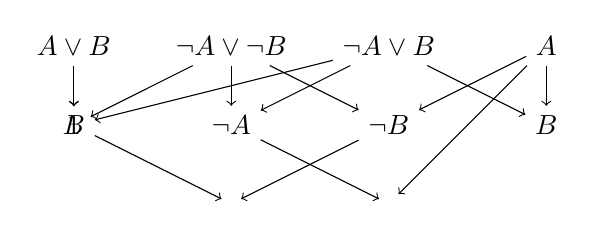
\begin{tikzpicture}[x=2cm]
\node (ab) at (0,10) {$A\vee B$};
\node (nanb) at (1,10){$\neg A\vee \neg B$};
\node (nab) at (2,10) {$\neg A \vee B$};
\node (a) at (3,10) {$A$};

\only<+>{
\node (1) at (0,9) {$1$};
\path (ab) edge[->] (1);
\path (nanb) edge[->] (1);
}

\uncover<+->{
\node (b) at (0,9) {$B$};
\path (ab) edge[->] (b);
\path (nab) edge[->] (b);
}

\uncover<+->{
\node (na) at (1,9) {$\neg A$};
\path (nanb) edge[->] (na);
\path (nab) edge[->] (na);
}

\uncover<+->{
\node (nb) at (2,9) {$\neg B$};
\path (nanb) edge[->] (nb);
\path (a) edge[->] (nb);
}

\only<+>{
\node (b1) at (3,9) {$ B$};
\path (nab) edge[->] (b1);
\path (a) edge[->] (b1);
}

\uncover<+->{
\node (e1) at (1,8) {$\square$};
\path (b) edge[->] (e1);
\path (nb) edge[->] (e1);
}

\uncover<+->{
\node (e2) at (2,8) {$\square$};
\path (na) edge[->] (e2);
\path (a) edge[->] (e2);
}


\end{tikzpicture}
}
\end{frame}

\end{document}
